% \begin{wrapfigure}[10]{hR!}{0.36\textwidth}
%     \vspace{-1.em}
%     \includegraphics[width=\linewidth]{pictures/files/samediffruns_m_soup.png}%
%     \caption{\textbf{Out-of-distribution accuracies on OfficeHome}. Averaging weights from multiple runs works better.}
%     \label{fig:soup:samediffruns_m_soup}%
% \end{wrapfigure}%
\begin{figure}[H]
    \vspace{-1.em}
    \centering
    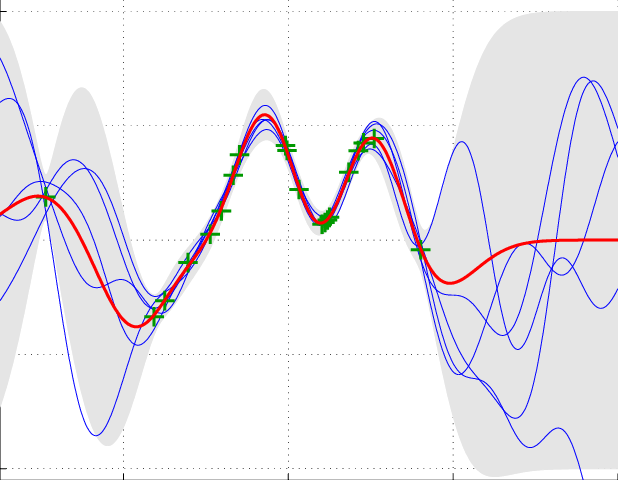
\includegraphics[width=0.4\textwidth]{pictures/files/final/gaussianprocess.png}%
    \caption{\textbf{Mean and variance of a Gaussian process's prediction}. Image from \cite{perez2013gaussian}. Intuitively, variance grows when samples are distant from training samples.}
    \label{fig:gp}%
\end{figure}%